% 1977 年辽宁卷第五题证法三：对角线 AC、BD 交于 O，∠1=∠2、∠3=∠4（内错角）
% （按源卷第 4 页「第五题 证法三附图」布局）
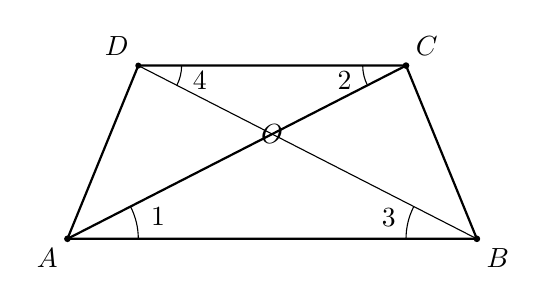
\begin{tikzpicture}[scale=1.0]
  \coordinate (A) at (0,0);
  \coordinate (B) at (5.2,0);
  \coordinate (D) at (0.9,2.2);
  \coordinate (C) at (4.3,2.2);
  \draw[thick] (A)--(B)--(C)--(D)--cycle;
  \draw[thick] (A)--(C);
  \draw[thin] (B)--(D);
  \draw[thin] ([shift={(A)}]0:0.9) arc[start angle=0,end angle=27.1,radius=0.9];
  \draw[thin] ([shift={(C)}]180:0.55) arc[start angle=180,end angle=207.1,radius=0.55];
  \draw[thin] ([shift={(B)}]152.9:0.9) arc[start angle=152.9,end angle=180,radius=0.9];
  \draw[thin] ([shift={(D)}]-27.1:0.55) arc[start angle=-27.1,end angle=0,radius=0.55];
  \node at (1.15,0.28) {$1$};
  \node at (3.52,2.01) {$2$};
  \node at (4.08,0.27) {$3$};
  \node at (1.68,2.01) {$4$};
  \node at (2.60,1.33) {$O$};
  \fill (A) circle (1.2pt) node[below left] {$A$};
  \fill (B) circle (1.2pt) node[below right] {$B$};
  \fill (D) circle (1.1pt) node[above left] {$D$};
  \fill (C) circle (1.2pt) node[above right] {$C$};
\end{tikzpicture}
